\documentclass[nobib]{tufte-handout}
\usepackage[english]{babel}
\usepackage{amsthm}
\usepackage{mathtools}
\usepackage{amsmath}
\usepackage{graphicx}

\newtheorem{definition}{Definition}
\newtheorem{lemma}{Lemma}
\newtheorem{theorem}{Theorem}
\newtheorem{xca}{Exercise}

\DeclarePairedDelimiter\floor{\lfloor}{\rfloor}
\title{Lecture 12: Vertex colouring $\cdot$ 1MA020}

\author[Vilhelm Agdur]{Vilhelm Agdur\thanks{\href{mailto:vilhelm.agdur@math.uu.se}{\nolinkurl{vilhelm.agdur@math.uu.se}}}}

\date{27 November 2023}


%\geometry{showframe} % display margins for debugging page layout

  \setkeys{Gin}{width=\linewidth,totalheight=\textheight,keepaspectratio}
  \graphicspath{{graphics/}} % set of paths to search for images
\usepackage{booktabs} % book-quality tables
\usepackage{units}    % non-stacked fractions and better unit spacing
\usepackage{multicol} % multiple column layout facilities
\usepackage{lipsum}   % filler text
\usepackage{fancyvrb} % extended verbatim environments
\fvset{fontsize=\normalsize}% default font size for fancy-verbatim environments

\usepackage{color,soul} % Highlights for text

% Standardize command font styles and environments
\newcommand{\doccmd}[1]{\texttt{\textbackslash#1}}% command name -- adds backslash automatically
\newcommand{\docopt}[1]{\ensuremath{\langle}\textrm{\textit{#1}}\ensuremath{\rangle}}% optional command argument
\newcommand{\docarg}[1]{\textrm{\textit{#1}}}% (required) command argument
\newcommand{\docenv}[1]{\textsf{#1}}% environment name
\newcommand{\docpkg}[1]{\texttt{#1}}% package name
\newcommand{\doccls}[1]{\texttt{#1}}% document class name
\newcommand{\docclsopt}[1]{\texttt{#1}}% document class option name
\newenvironment{docspec}{\begin{quote}\noindent}{\end{quote}}% command specification environment



\begin{document}    
\include{mathcommands.extratex}
\maketitle% this prints the handout title, author, and date

\begin{abstract}
\noindent
We study the notion of a vertex colouring of a graph, and prove some results about the chromatic number of a graph. We prove Brooks' theorem, the five-colour theorem for planar graphs, and the three-colour theorem for outerplanar graphs. We use the latter to prove the art gallery theorem.
\end{abstract}

\section{Introductory results}

We already saw the notion of colouring a graph in an earlier lecture, but we proved nothing about it other than some very basic bounds. Let us restate the definition, and then move on to proving some more interesting things.
\begin{marginfigure}
    \centering
    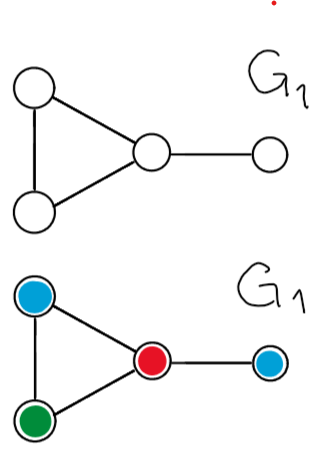
\includegraphics[width=0.9\textwidth]{k-coloring.png}
    \caption{
    Example of an undirected graph $G_1$ that is three-coloured. In this case the chromatic number of $G_1$ is $\chi(G_1)=3$ since we can find a three-colouring of $G_1$ but not a two-colouring.
    }
\end{marginfigure}
\begin{definition}
  A \emph{$k$-colouring} of a graph $G = (V,E)$ is a function $c: V \to [k]$, where we think of the numbers $1,2,\ldots,k$ as colours, such that no two adjacent vertices are sent to the same colour.\sidenote[][]{On rare occasions, we will want to think about colourings that do not necessarily fulfill this condition. Then we will call those colourings \emph{improper}, and the ones with the property will be \emph{proper colourings}.} The \emph{chromatic number} of a graph $G$, denoted $\chi(G)$, is the least integer $k$ such that $G$ has a $k$-colouring.
\end{definition}

In order to upper bound the chromatic number of a graph, the most obvious approach is of course to construct a colouring of it. The most straightforward way to do this is greedily:

\begin{definition}
  Let $G = (V,E)$ be a graph with an ordering on the vertices, say $v_1 < v_2 <\ldots<v_n$. On the colours, we use the obvious ordering $1 < 2 < \ldots$. The \emph{greedy colouring algorithm} starts with an empty colouring, and then at each time-step, it colours the first uncoloured vertex (according to the ordering on the vertices) with the first colour that has not been used on any of its neighbours.
\end{definition}

If we do nothing special in the choice of ordering of vertices, we don't get any very strong bound from this, of course. We do, however, get the following general bound:

\begin{lemma}\label{lemma:trivial_chi_upper_bound}
  For any graph $G$ with maximum degree $\Delta$, we have
  $$\chi(G) \leq \Delta + 1.$$

  \begin{proof}
    Pick an arbitrary ordering on the vertices, and run the greedy colouring algorithm. For any vertex, when it is about to be coloured, it has at most $\Delta$ neighbours that already have colours, and so one of the first $\Delta + 1$ colours must be unused.
  \end{proof}
\end{lemma}

If we know something about the graph, we can be a bit more clever in our choice of ordering, and get a better bound. To do this, however, we first need to define the breadth-first ordering of the vertices of a graph.
\begin{marginfigure}
    \centering
    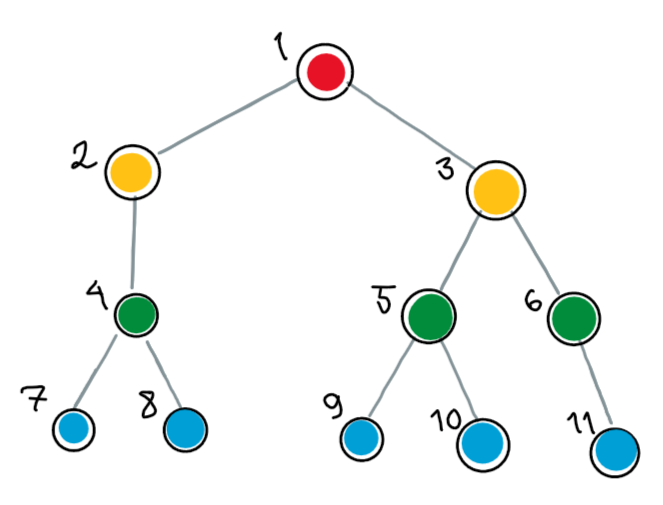
\includegraphics[width=0.9\textwidth]{BFS_visualization.png}
    \caption{
    This is a visualization of the order that we visit each vertex in a graph using Breadth-first search.
    }
\end{marginfigure}
\begin{definition}
  Let $G = (V,E)$ be a graph. \emph{Breadth-first search} started at a vertex $v$ proceeds as follows:
  \begin{enumerate}
    \item Initialize the \emph{currently visited vertex} to $v$, the list of \emph{discovered vertices} $D$ to be empty, and the list of \emph{visited vertices} $W$ to be empty.
    \item Add all the neighbours of the currently visited vertex to the end of $D$, in an arbitrary order.
    \item Add the currently visited vertex to the end of $W$.
    \item If $D$ is not empty, remove the first element of $D$, and let it be the new currently visited vertex. Otherwise, return $W$.
  \end{enumerate}

  This algorithm will return a list of the vertices of the connected component containing $v$. The order in which these vertices appear is called a \emph{breadth-first ordering} of the vertices, started at $v$. 
  
  We could also modify the algorithm slightly, to make each vertex remember which vertex was the currently visited one when it was added to the list of discovered vertices. Then we get a \emph{breadth-first spanning tree} rooted at $v$ by having each vertex consider its parent as the vertex that discovered it.
\end{definition}

\begin{lemma}\label{lemma:brooks_for_irregular}
  Suppose $G$ is a graph with maximum degree $\Delta$, whose vertices do not all have the same degree. Then
  $$\chi(G) \leq \Delta.$$

  \begin{proof}
    Since not all vertices have the same degree, there must exist a vertex $v$ with $d_v < \Delta$. Now order the vertices of $G$ according to the \emph{inverse} of the breadth-first order on the vertices started at $v$,\sidenote[][]{By assumption $G$ is connected, so the breadth-first search will find every vertex.} and run the greedy colouring algorithm with this ordering.

    The crucial property we need from the ordering is that every vertex except $v$ will, when visited by the greedy colouring algorithm, have at least one neighbour that has not yet been coloured. So it has at most $\Delta - 1$ coloured neighbours, and so there is always at least one colour available among the first $\Delta$ colours.

    When we finally get to $v$, it has degree less than $\Delta$, so it too has fewer than $\Delta$ coloured neighbours, and can pick a colour from among the first $\Delta$.
  \end{proof}
\end{lemma}

We can also make use of our previous work on connectivity to break down the problem of finding a colouring of a graph into finding a colouring of its two-connected blocks.

\begin{lemma}\label{lemma:chi_max_over_biconnecteds}
  Suppose $G$ is some graph which has at least one two-connected block, and let $B_1, B_2, \ldots, B_r$ be its collection of two-connected blocks. Then
  $$\chi(G) = \max_{i\in[r]} \chi(B_i).$$

  If $G$ has no two-connected blocks, $\chi(G) = 2$ if $G$ has at least one edge, and $\chi(G) = 1$ if it has no edges.\sidenote[][-0.5cm]{
    \begin{xca}
      Prove this part of the theorem statement.
    \end{xca}}
\end{lemma}

  \begin{proof}
    That the chromatic number of $G$ is lower bounded by the max over the blocks is trivial. To see the other direction, consider the block graph of $G$, which we saw in our previous lecture is a forest.

    Colour each block of $G$, using at most $\max_{i\in[r]} \chi(B_i)$ colours.\sidenote[][]{If the block is two-connected, this is trivially possible. Otherwise it can be coloured with at most two-colours, since it must be an isolated vertex or a $K_2$.} Then, because any two blocks only intersect in at most one vertex, we can permute the colours in each block so that they agree on the cutvertices, and this can be done in such a way that we get a colouring on the entire graph because the block graph is a tree.\sidenote[][]
    {\begin{xca}
      Write out the details of this argument -- how do you actually algorithmically do this?
    \end{xca}} 
    Clearly permuting the colours does not add new colours, so our global colouring will also use only $\max_{i\in[r]} \chi(B_i)$ colours.
  \end{proof}


\section{Brooks' theorem}

When we first introduced the notion of a colouring of a graph, we found an example where Lemma \ref{lemma:trivial_chi_upper_bound} is actually sharp: For the complete graph, we have $\chi(K_n) = n = \Delta(K_n) + 1$. There is also another example, namely the cycle graphs of odd length, which have chromatic number three and maximum degree two.

Are there any other cases where this inequality is sharp? It turns out that these are in fact the only connected examples, which is the content of Brooks' theorem.

\begin{theorem}[Brooks, 1941]
  Let $G$ be a finite connected graph with maximum degree $\Delta$ that is not complete nor a cycle of odd length. Then
  $$\chi(G) \leq \Delta.$$

  \begin{proof}
    If $G$ is not regular, then the theorem follows from Lemma \ref{lemma:brooks_for_irregular}, so we can assume that all vertices of $G$ have degree $k$. Now, obviously, the only $1$-regular connected graph is $K_1$, and we have assumed $G$ is not complete.

    For $k=2$, the only connected $2$-regular graphs are the cycles. We have assumed $G$ is not a cycle of odd length, and we know the cycles of even length have chromatic number $2$.

    So we may assume $k \geq 3$. We may additionally, by Lemma \ref{lemma:chi_max_over_biconnecteds}, assume that $G$ is at least two-connected. So we now divide into two cases:

    Suppose $G$ is in fact also three-connected. Then, since $G$ is not complete, we can find three vertices $a, v, b$ such that $a \sim v, b \sim v \in E$, but $a$ and $b$ are non-adjacent. Since $G$ is three-connected, the graph $G[V\setminus \{a,b\}]$ is connected.

    We can now colour $G$ in a way similar to what we did for Lemma \ref{lemma:brooks_for_irregular}. First, we let $a$ and $b$ both take the colour $1$, which is possible since they are non-adjacent. Then we run the greedy colouring algorithm on the rest of the vertices using the inverse of a breadth-first search order started at $v$.

    Again, each vertex other than $v$ will have fewer than $k$ already-coloured neighbours when it is visited,\sidenote[][]{Even taking into account that $a$ and $b$ already have a colour -- think about why this is true.} so they can be coloured using only $k$ colours, as before. Now, $v$ will have all of its $k$ neighbours coloured -- however, two of those neighbours, $a$ and $b$, have the same colour, so its neighbours are using fewer than $k$ \emph{distinct} colours, so there is one left over for $v$.

    So for the other case, suppose that in fact $\kappa(G) = 2$. Now, if we could find a triple of vertices $a, v, b$ with the same properties as in the three-connected case, that argument would of course work again -- so we need a new argument for why such a triple exists.

    So let $a$ be an arbitrary vertex of $G$. If $G[V \setminus \{a\}]$ is still $2$-connected, we can pick $x$ as any neighbour of $a$ and $b$ as any neighbour of $x$ other than $a$, and these will have the required properties.

    \begin{marginfigure}
      \centering
      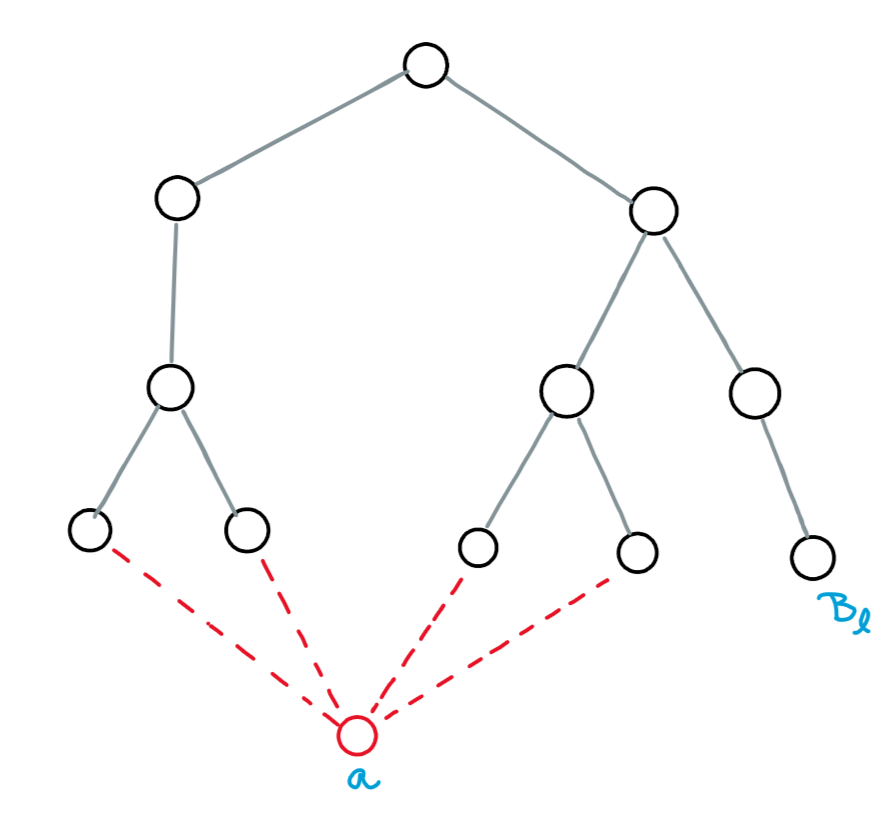
\includegraphics[width=0.9\textwidth]{brooks_theorem_blocktree.png}
      \caption{A sketch of the block graph of $G[V \setminus \{a\}]$ and the vertex $a$ drawn in in red, with dotted edges connecting it to blocks it is in as a non-cutvertex, and the putative but impossible leaf $B_\ell$ that does not contain $a$. Notice how the addition of $a$ will create cycles forcing everything except $B_\ell$ to become a single block. Also notice how $a$ being the cutvertex in $B_\ell$ wouldn't help -- that would create a dotted line from $a$ to the parent of $B_\ell$, which still does not create a cycle with $B_\ell$ in it.}
    \end{marginfigure}

    Now, if $G[V \setminus \{a\}]$ is not two-connected, we claim that its block graph must be a tree with at most $k$ leaves, and each of these leaves is a block $B_i$ which contains a non-cutvertex $b_i$ which is adjacent to $a$ in $G$. 
    
    If this were not the case, there would be some block $B_\ell$ such that adding $a$ back in did not create a cycle intersecting $B_\ell$ in at least two vertices, and so $B_\ell$ would still be a separate block in $G$. But $G$ is two-connected, so this is impossible.
    
    Now we pick $a$ as the central vertex and $b_1$ and $b_2$, say, as the other two vertices. To see that this is a triple of vertices with the right properties, we need to see that $b_1$ and $b_2$ are non-adjacent. Now, we know that if they were adjacent they would be in the same block, but we also also know they are not cutvertices and so belong to only one block, and by assumption they are in the distinct blocks $B_1$ and $B_2$. So they are not adjacent, and we have found a triple with the right properties, finishing the proof.
  \end{proof}
\end{theorem}

\section{Colouring planar graphs}

One of the perhaps more famous theorems of graph theory is that any map can be coloured in at most four colours. Of course, part of the reason this is famous is because it has only been proved by means of a computer checking many many cases, so in a sense no human has ever understood an entire proof.

However, the weaker statement that any planar graph can be coloured with \emph{five} colours can be proven much more easily. In fact, the proof we will give is a modification of a flawed early ``proof'' of the four-colour theorem from the late nineteenth century.

\begin{theorem}
  For any planar graph $G$, $\chi(G) \leq 5$.

  \begin{proof}
    We prove this by induction in the number of vertices. The base case of the one-vertex graph is trivial.

    For the inductive step, let $v$ be a vertex whose degree in $G$ is minimal. We claim that $d_v \leq 5$.\sidenote[][]{This follows from the inequality $$|E| \leq 3|V| - 6$$ which we proved last lecture.} Now, if we let $G' = G[V \setminus \{v\}]$, this is clearly still planar and has fewer vertices, so by our induction hypothesis we can five-colour it.

    If $d_v \leq 4$, its neighbours only use at most four colours, so there's a fifth colour available for us to give it. So we may assume $d_v = 5$. If $v$ has two neighbours which have the same colour, there is again an unused colour we can assign to it. So we assume all five neighbours have different colours.

    Now, if we fix a planar embedding of $G$, we can call $v$'s five neighbours $v_1, v_2, \ldots, v_5$ in clockwise order, and we can relabel our colours so that $v_i$ has colour $i$ for each $i$.

    Let $G(1,3)$ be the induced subgraph of just vertices coloured $1$ or $3$, as we did in the exercise about Kempe chains. If $v_1$ and $v_3$ are in different Kempe chains, that is, in different connected components of $G(1,3)$, we can do a Kempe change, swapping the two colours in one of the connected components, so that $v_1$ and $v_3$ have the same colour. After doing this, one colour will of course have become available for $v$, and so we can finish our colouring.

    \begin{figure}
      \centering
      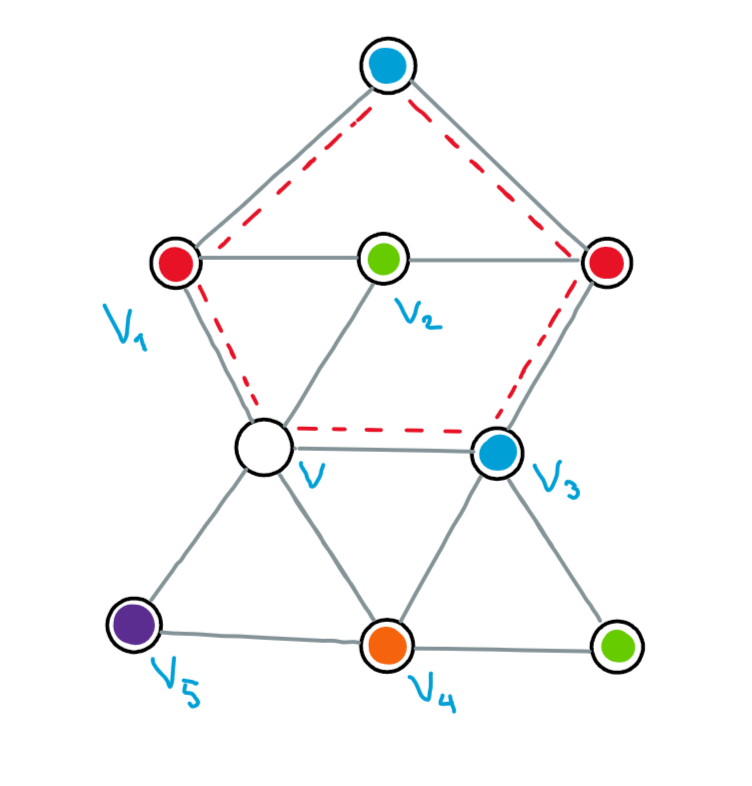
\includegraphics[width=0.65\textwidth]{planar_five_colour.png}
      \caption[][0cm]{An illustration of the situation in the proof of the five-colour theorem. $v_1$ and $v_3$ are in the same $(\text{red},\text{blue})$-component, which forces the existence of the cycle indicated by a dashed red line. This cycle, however, separates $v_2$ and $v_4$ into separate $(\text{green},\text{orange})$-components, so $v_4$ can swap its orange colour with the green of its neighbour. This frees up the colour orange for $v$ to use.}
      \label{fig:planar_five_colour}
    \end{figure}

    So suppose instead that $v_1$ and $v_3$ are in the same $(1,3)$-component. Then there exists a path $P$ from $v_1$ to $v_3$, not using $v$, all of whose vertices are coloured $1$ or $3$. This path, together with the path $v_1\, v\, v_3$, forms a cycle, which separates $G$ into an inside and an outside.

    By construction, $v_2$ has to lie on the inside of the cycle, and $v_4$ on the outside. So in particular they must be in different $(2,4)$-components, and so we can apply a Kempe change to these two components, freeing up a colour for $v$ just as before.
  \end{proof}
\end{theorem}

\section{The art gallery theorem and outerplanar graphs}

Consider the following problem: We are given an arbitrary simple polygon\sidenote[][]{It being \emph{simple} means that it contains no holes and no two sides intersect.} in the plane, which we interpret to be an art gallery. We want to post guards in the gallery to watch over every point of the gallery, to prevent any climate activists from throwing tomato soup on the art. How many guards do we need?

We will prove the following theorem:

\begin{theorem}
  For any art gallery (simple polygon) with $n$ corners, we need at most $\floor{\frac{n}{3}}$ guards to watch the entire gallery.
\end{theorem}

The first step to proving this is of course to turn the simple polygon into a graph.\sidenote[][]{Since, of course, if the solution didn't involve graphs, the problem wouldn't be in this course.} We do this by first triangulating the polygon, and then interpreting each corner as a vertex and each line as an edge, as illustrated in Figure \ref{fig:triangulated_polygon}.

\begin{figure}
  \centering
  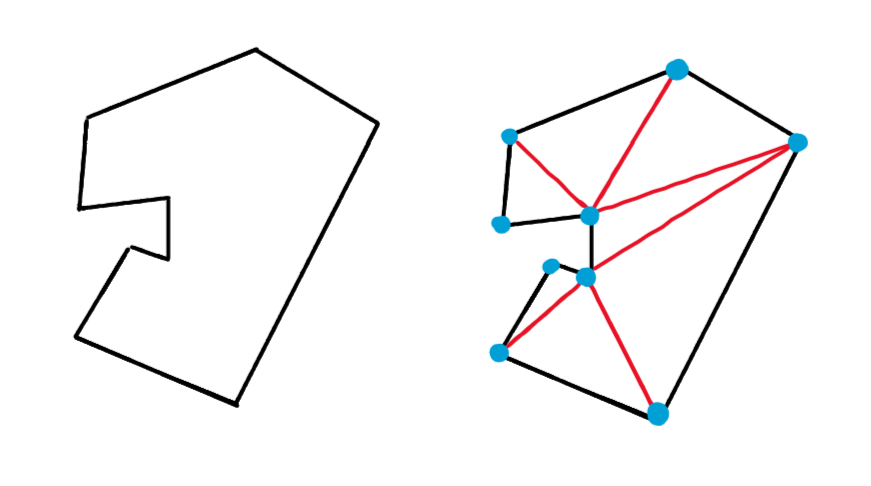
\includegraphics[width=0.65\textwidth]{triangulated_polygon.png}
  \caption[][0cm]{A simple polygon on the left, and a triangulated version on the right, which we can interpret as a graph with corners as vertices, and the black and red lines as edges.}
  \label{fig:triangulated_polygon}
\end{figure}

We can make two observations about the resulting graph, one obvious and one less immediately obvious. The first is that this graph is planar and comes with an obvious embedding, from how we drew the polygon. The second is that in fact all the vertices of this graph are incident to the unbounded face -- there are no vertices on the ``inside'' of the graph.

There is in fact a name for the class of graphs that have this second property:

\begin{definition}
  A graph $G$ is called \emph{outerplanar} if there exists a planar embedding of it in which all the vertices are incident to the unbounded face.
\end{definition}

For these graphs, we can do a lot better than the five-colour theorem we proved earlier.

\begin{theorem}
  All outerplanar graphs are three-colourable.

  \begin{proof}
    By Lemma \ref{lemma:chi_max_over_biconnecteds} it suffices to prove this for two-connected outerplanar graphs, for which we prove it by induction on the number of vertices. 
    
    The base case of $|{V}| = 1$ is trivial, so let $G$ be an outerplanar graph on $n \geq 2$ vertices. Since adding edges cannot decrease the chromatic number or connectivity, we may assume that $G$ is in fact edge-maximal two-connected outerplanar. This implies that all faces are triangles, since any face that isn't could be subdivided into triangles by adding an additional edge, while still leaving the graph two-connected outerplanar.

    We claim that the planar dual of $G$ with the unbounded face deleted\sidenote[][]{This is called the \emph{weak planar dual} of $G$.} is a forest,\sidenote[][]{In fact it will be connected, since we assumed $G$ is two-connected, but we don't need this here.} since if there were a cycle in the weak planar dual, this cycle would enclose a vertex of $G$, which would then not be incident to the unbounded face.

    So let $f$ be some leaf of the weak planar dual. We know that this face is a triangle, and since it is a leaf, and thus only incident to at most one other bounded face, it must contain a vertex $v$ incident only to $f$ and the unbounded face.\sidenote[][]{This is where we use the assumption that $G$ is two-connnected: If it were not, $v$ could be a cutvertex of $G$, and thus actually sit in two different faces despite $f$ being a leaf of the weak planar dual.} In particular, $d_v = 2$.

    If we delete $v$ from $G$, we get a smaller graph that is still outerplanar, and so by induction it is three-colourable. Now $v$ only has two neighbours in this graph, and so we can colour $v$ with the third colour unused by both its neighbours.
  \end{proof}
\end{theorem}

How does this give us a proof of the art gallery theorem? Well, what we have seen is that we may three-colour the corresponding graph, and of course any colour class of this colouring must contain one vertex from each triangle. So if we post a guard at all the red vertices, each triangle is seen by one of these guards, and thus the entire graph is seen.

\section{Exercises}

\begin{xca}
  In this exercise, we use some \emph{spectral} methods for deriving results about the chromatic number. We rely on the following lemma, which can be proved using the technique of Rayleigh-quotients:

  \begin{lemma}
    Let $G$ be a graph and $H$ an induced subgraph of $G$, and let their adjacency matrices be $A_G$ and $A_H$ respectively. Then
    $$\lambda_{\min}\left(A_G\right) \leq \lambda_{\min}\left(A_H\right) \leq \lambda_{\max}\left(A_H\right) \leq \lambda_{\max}\left(A_G\right),$$
    and
    $$\delta(G) \leq \lambda_{\max}\left(A_G\right) \leq \Delta(G),$$
    where $\delta(G)$ and $\Delta(G)$ are the minimum and maximum degree of $G$.
  \end{lemma}

  Use the above lemma to prove the below theorem:
  \begin{theorem}[Wilf, 1967]
    For any graph $G$ with adjacency matrix $A_G$, we have
    $$\chi(G) \leq \lambda_{\max}\left(A_G\right) + 1.$$
  \end{theorem}

  \textbf{Hint:} Let $H$ be a minimal induced subgraph of $G$ with $\chi(H) = \chi(G)$. Can you relate the minimum degree of $H$ to the chromatic number of $G$?\sidenote[][]{If you want a solution, a full proof is in the lecture notes from last year.}
\end{xca}

\begin{xca}
Assume you have to separate English alphabet letters into boxes such that no two consecutive letters end up in the same box. What is the minimum number of boxes you need for this task?
\end{xca}

\begin{xca}
Prove that if a graph has at most two cycles of odd length then it can be
coloured with 3 colours. \textit{Hint}: a bipartite graph has $\chi(G) = 2$.
\end{xca}


%\bibliography{references}
%\bibliographystyle{plainnat}

\end{document}
